\chapter{Data and methods}
\label{ch:data_methods}
	In this chapter we describe our approach to achieve the research objectives stated during the introduction. The first section of this chapter introduces the datasets used during this study and the underlying causes for using them. For each dataset, we shortly describe by which approach it is derived and what are the fundamental meta-data properties. Additionally, if possible we try to give for each dataset an accuracy assessment, ideally provided by other research groups if available. Finally, we describe our idea behind using the data and how we acquired and filtered it. The second and last section of this chapter is focused on the applied methodology to prepare our analysis and results. For each processing step we give a short description of the methodical background and describe the core functionality of our processing algorithms. For implementing our processing algorithms and visualizing our results we selected individually the programming language or software which fulfills best our requirements. These approaches are encapsulated in a reusable software design to easily reproduce, alter or reuse our algorithms and findings.

\section{Data}
\label{sec:data}
	\begin{table}[ht]
		\centering
		\caption[Datasets used in this study]{\textbf{Datasets used in this study}}
		\label{tab:datasets}
		\begin{tabular}{lll}
			\hline
			Data & Type & Source \\\hline
			Global Forest Change & spatial & \citet{Hansen2013} \\
			GlobeLand30 & spatial & \citet{Chen2015} \\
			Aboveground Woody Biomass & spatial & \citet{Baccini2015} \\
			Intact Forest Landscape & spatial & \citet{Potapov2017} \\
			Global Soil Organic Carbon Content & spatial & \citet{FAO2018} \\
			Global Administrative Areas & spatial & \citet{Hijmans2018} \\
			Soil Organic Carbon Change & empirical & \citet{Don2010} \\
			\multirow{3}{*}{Ecosystem Service Values} & \multirow{3}{*}{empirical} & \citet{Costanza2014} \\
			&& \citet{Groot2012} \\
			&& \citet{Siikamaki2015} \\\hline
		\end{tabular}
	\end{table}
	The table \ref{tab:datasets} shows a comprehensive overview of the applied datasets for this study. Spatial datasets comprises vector as well raster data, while empirical data is extracted from the cited publications. The subsequent sections describe each dataset in further detail.

	\subsection{Global Forest Change}
	\label{subsec:methods_gfc}
		\ac{GFC} 2000-2012 Version 1.0 is the first high-resolution dataset that provides a comprehensive view of the annual global forest cover change between 2000 and 2012 \citep{Hansen2013,Li2017}. We will use this dataset to extract and determine the tropical deforestation and reforestation dynamics for our study time frame from 2000 till 2010. The initial \ac{GFC} dataset released by \citeauthor{Hansen2013} has been extended by recent releases, which encompass the annual forest cover changes between 2000-2013, 2000-2014, 2000-2015 and 2000-2016, respectively. All versions of this dataset are derived from growing-season imagery captured by the following remote sensing satellites: Landsat 7 ETM+, Quickbird, MODIS \citep{Hansen2013}. On the satellite imagery, a time-series spectral metrics analysis is applied to gather the global forest extent in 2000 as well as the annual forest loss and the accumulated gain for the period 2001-2012. Hence, \ac{GFC} comprises three independent data layers: tree cover, annual forest loss, and forest gain. Each of these layers is divided into 10x10 degree tiles by the \ac{CRS} \ac{WGS84} (EPSG:4326) with a spatial resolution of 1 arc-second per pixel or 30 m per pixel. Further, across the provided \ac{GTiff} layers the pixel data is coded in unsigned 8-bit integers. Hansen et al. defined trees as all vegetation taller than 5 meters. For each pixel covered by trees, a canopy density ranging from 0 to 100\% is computed. Forest loss is defined as a stand displacement disturbance leading from a forest state to a non-forest state (e.g. canopy density >50\% to 0). Resulting form this definition, the underlying causes of forest loss range from anthropogenic impacts to natural causes. Tree cover gain is defined as the inverse of loss, and the canopy density must exceed 50\% to get recognized.

		\citet{Hansen2013} reports a tree cover loss accuracy assessment of 83\% for the tropical region. The mapped tree cover gain achieves a producers accuracy of approximately 48\%, while the users accuracy is approximately 81\%. The large difference between users and producers accuracy highlights that tree cover gain is underestimated by the algorithm. For a part of the Riau province in Indonesia \citet{Arjasakusuma2018} reports for the gain layer a producers and users accuracy of 64.5\%$\pm$7\% and 75.9\%$\pm$8.1\%, respectively. By this independent validation the underestimate of tree cover gain is largely confirmed for this region. For Gabon \citet{Sannier2016} reports as accuracy assessment for the \ac{GFC} tree cover map an overall accuracy of 95.87\% and 96.6\% for the canopy density thresholds of >30\% and >70\%, respectively. In subtropical areas the \ac{GFC} dataset achieves an overall accuracy of 62\%, 64\%, 66\% for the canopy density thresholds of >10\%, >30\%, and >50\% \citep{McRoberts2016}.

		This dataset is publicly available for download without any constraint. For a convenient bulk download, the dataset homepage provides a "\verb|*.txt files|" comprising the \ac{URL} of the tiles for each sub-dataset. The spatial location of an image can be directly determined from the file name within the \ac{URL}. Each file name has a common pattern shown by the following expression: "\verb|Hansen_VERSION_LAT[NS]_LNG[WE]|". LAT (latitude) and LNG (longitude) refer to the top left corner coordinates of a raster image, whereas these coordinates are only given in natural numbers. The orientation of the image on the hemisphere is determined by the four cardinal directions N (north), S (south), W (west) and E (east). For this project, we require all three sub-datasets, namely: Treecover2000, loss-year, and gain. The data acquisition is automatized with a Python script by using the standard-library modules urllib and re. At first, the Python script downloads the provided "\verb|*.txt|" files and creates a list data structure, where each \ac{URL} is an element of this list. After, it cycles through the list and extracts the corner coordinates from the file name by means of a REGEX (Regular Expression). These corner coordinates and cardinal directions are converted to valid latitude and longitude coordinates between $[-90, 90]$ and $[-180, 180]$, respectively. Now, an image is only downloaded if it is within the study extent between $[-20, 30]$ latitude. The acquired image tiles in total 678 are shown in the top panel (green squares) in figure \ref{fig:dataset_tiles}.
		\begin{figure}[ht]
			\centering
			\includegraphics[scale=.93]{img/tiles}
			\caption[Map of dataset tiles]{\textbf{Map of downloaded dataset tiles:} This map shows the acquired image tiles used for this study. From top to bottom Global Forest Change (GFC) dataset tiles (Treecover2000, loss-year and gain) (green), the land cover dataset GlobeLand30 (GL30) tiles (red), and the Aboveground Biomass (AGB) dataset tiles (blue). The orange filled shapes highlight countries within the tropical zone.}
			\label{fig:dataset_tiles}
		\end{figure}

	\subsection{GlobeLand30}
		\ac{GL30} is the first global land cover dataset with 30 meter spatial resolution that provides a comprehensive view on the distribution of 10 different land cover classes (table \ref{tab:gl30_classes}) over the entire globe \citep{Chen2017}. We will use this dataset to classify tree cover loss and subsequently derive the \acp{PDD} of tropical forest. Currently, this dataset is available for two different time steps 2000 and 2010 \citep{Chen2015}. The pixel values of this dataset are coded in unsigned 8-bit integers and as \ac{CRS}, it uses \ac{WGS84} in \ac{UTM} projection. \ac{GL30} can be downloaded as a \ac{GTiff} raster mosaic where each image covers 6x5 degrees \citep{Chen2014}. For detecting the land cover classes \citeauthor{Chen2015} used a so-called Pixel-Object-Knowledge oriented approach and satellite imagery from Landsat ETM+ \citep{Chen2015}. The mapping process was divided into different stages where each land cover type is detected separately and deleted subsequently from the source image. The applied mapping order is the following: water bodies, wetland, snow and ice, cultivated land and forest, shrubland, grassland and bare land synchronous. To detect the pixels of a selected land cover type the following pixel-level classifiers are used: Decision Trees, Support Vector Machines or Maximum Likelihood Classifier. After pixel detection, the adjacent pixels are grouped as an aggregated land use object. These objects are subsequently validated by expert knowledge and the gained knowledge is used as a feedback loop to improve the automatized classification.

		\citet{Chen2015} estimates an overall mapping accuracy of 80.33 \% and 78.6 \% for 2000 (only validated in Shaanxi, China) and 2010 (global), respectively. Several research groups besides \citeauthor{Chen2015} validated the mapping accuracy of \ac{GL30} at different regions and scales. \citeauthor{Arsanjani2016} estimates an overall accuracy of 77.9 \% for Iran and an accuracy of >80 \% is reported for Germany \citep{Arsanjani2016a,Arsanjani2016}. \citet{Yang2017}, \citet{Cao2016} and \citet{Jacobson2015} estimate the accuracy of 82.4 \%, 80.1 \% and 83.1 \% for China, Nepal, and East Africa, respectively. To the best of our knowledge, no study have focused on validating the mapping accuracy for regions exclusively within the tropical zone.

		\citeauthor{Chen2015} donated the \ac{GL30} land cover mapping to the UN (United Nations) but it is not accessible for public download unless the user registers on the dataset homepage. A registered user must fill an order application to get access to the image tiles. The application form must contain the tile identifiers and the selected time period. Tile identifiers have the following common pattern: "\verb|[NS]ZONE_LAT_NAME|" where zone refers to the \ac{UTM} zone between $[1, 60]$, N (north) or S (south) to the cardinal direction, and LAT (latitude) to the latitude coordinate of the top left corner. On the dataset homepage a vector file can be downloaded which contains the dataset tile polygons with assigned identifiers. This file was used to select all required tiles within the tropical zone between approximately $[-23, 23]$ degrees (\ac{WGS84}). Figure \ref{fig:dataset_tiles} presents the selected images (middle panel-red). The corresponding image identifiers are converted to a single line string and copied to the application form. After submitting the form the order will be checked and approved within two weeks. After one week we received a two weeks limited access to a password protected FTP-server where we downloaded 716 raster images. Due to the several restrictions, this process of selecting and downloading could not be automatized with one pipeline. Only the selection and string conversion were automatized with a throwaway script.
		\begin{table}[ht]
			\centering
			\caption[Land cover classification of the GlobeLand30 product]{\textbf{Land cover classification of the GlobeLand30 product:} The code column is the assigned pixel value, type refers to the corresponding land cover type and definition explains in broad terms which types of surfaces fall into each land cover type \citep{Chen2017}.}
			\label{tab:gl30_classes}
			\begin{tabular}{rlp{10.3cm}}
				\hline
				Code & Type & Definition \\\hline
				10 & Cultivated land & Used for agriculture, horticulture and gardens, including paddy fields, irrigated and dry farmland, vegetable and fruit gardens, etc. \\
				20 & Forest & Covered by trees, vegetation covers over 30\%, including deciduous and coniferous forest, and sparse woodland with cover 10-30\%, etc. \\
				30 & Grassland & Covered by natural grass with cover over 10\%, etc.\\
				40 & Shrubland & Covered by shrubs with cover over 30\%, including deciduous and evergreen shrubs, and desert steppe with cover over 10\%, etc.\\
				50 & Wetland & Covered by wetland plants and water bodies, including inland marsh, lake marsh, river floodplain wetland, forest/shrub wetland, peat bogs, mangrove and salt marsh, etc.\\
				60 & Water bodies & In land area, including river, lake, reservoir, fish pond, etc.\\
				70 & Tundra & Covered by lichen, moss, hardy perennial herb and shrubs in the polar regions, including shrub-, herbaceous-, wet- and barren-tundra, etc.\\
				80 & Artificial surfaces & Modified by anthropogenic influence, including all kinds of habitation, industrial and mining area, transportation facilities, and interior urban green zones and water bodies, etc.\\
				90 & Bareland & With vegetation cover lower 10\%, including desert, sandy fields, Gobi, bare rocks, saline and alkaline land, etc.\\
				100 & Snow and ice & Covered by permanent snow, glacier and icecap\\\hline
			\end{tabular}
	\end{table}

	\subsection{Aboveground Live Woody Biomass Density}
		The \ac{AGB} raster dataset is prepared by \ac{GFW} by an adapted approach of \citet{Baccini2012,Baccini2015,Baccini2017}. We will use this raster dataset to determine \ac{AGB} losses by \acp{PDD} of the tropical tree cover. For the year 2000, this dataset estimates the aboveground biomass density per pixel in Mg biomass ha$^{-1}$ (megagram biomass per hectare), and the confidence per pixel at a spatial resolution of approximately 1 arc-second or 30 m. The dataset covers the global tropical zone as a mosaic of \ac{GTiff} raster images, where each tile of the mosaic has the \ac{CRS} \ac{WGS84} and is coded in a float. For deriving biomass density \ac{GFW} used canopy metrics from GLAS LIDAR (Geoscience Laser Altimeter System Light Detection and Ranging) footprints and several regional and forest-specific allometric equations. The resulting GLAS \ac{AGB} estimates are used as predictor variables to train regional-specific random forest models based on Landsat 7 ETM+ top-of-atmosphere reflectance, tree canopy density of \ac{GFC}, elevation data, and climate data as predictor variables. Next, these models are subsequently applied to the entire study extent to predict the biomass content for each pixel. Additionally, an uncertainty layer is prepared accounting for the errors from allometric equations, the LIDAR-based model, and the random forest model.

		The \ac{AGB} raster mosaic is publicly available on the homepage of \ac{GFW}. As mentioned, the dataset covers only the tropical zone, therefore we acquire the entire mosaic. The \ac{GFW} homepage provides an \ac{API} to receive the actual \ac{URL} of each raster image. If a request is sent to this \ac{API} the server responded with a GeoJSON (Geographic JavaScript Object Notation) feature collection. The collection contains as attributes the \acp{URL} of the biomass images, the \acp{URL} of the uncertainty layers, and the rectangular bounds of each image. The data acquisition is automatized by means of Python and the standard-library modules urllib, threading, and the open source library geopandas. At first, the GeoJSON is downloaded via an \ac{API} call and eventually stored on disk. Next, we iterate the features of the GeoJSON collection and extract the \ac{URL}s (biomass and uncertainty) of each tile. These \ac{URL}s are downloaded and subsequently stored on disk. During the downloads of the uncertainty layers, the \ac{GFW} server answered repeatedly with a 404 (Not found). Therefore the uncertainty layers are not available. In total we downloaded 105 different image tiles, their extent and spatial location are shown in blue at the bottom panel of figure \ref{fig:dataset_tiles}.

	\subsection{Intact Forest Landscapes}
		An \ac{IFL} is defined as a mosaic of undisturbed forest patches or a naturally treeless ecosystems without signs of human activity and large enough to maintain all native biological diversity \citep{Potapov2017}. We will use this dataset to distinguish between deforestation in primary or secondary forest to decide which \ac{SOC} change coefficient from section \ref{subsec:methods_socc} will be selected. On the fact that \ac{IFL} comprises different intact natural landscape patterns like primary forests, non-forest ecosystems, temporary treeless areas after a natural disturbance, and water bodies the term is not congruent to the term primary forest defined by the \ac{FAO} \citep{FAO2012}. However, as mentioned \ac{IFL}s includes large patches of primary forests with a minimum extent of 500 Km$^2$, therefore, primary forests can be extracted from the layer. Still, there are smaller fragments of primary forest outside of the \ac{IFL}s. In regards to the extent, an \ac{IFL} has a minimum size of 500 Km$^2$, a minimum width of 10 Km, and a minimum corridor/appendage width of 2 Km. Further an \ac{IFL} should not contain any of the following: ecosystem alternation, fragmentation by infrastructure and disturbance, and areas altered or managed through agriculture, logging, and mining. For mapping and detecting \ac{IFL}s \citeauthor{Potapov2017} used Landsat imagery and several auxiliary data sources like \ac{GFC}, and national transportation maps. The dataset can be downloaded as a \ac{SHP} file with the coordinate reference system \ac{WGS84}. Each polygon in the \ac{SHP} represents an \ac{IFL} patch at a certain location on our planet at the time period 2000.

		Data acquisition is pretty straight forward, since the \ac{IFL} dataset is publicly accessible for download. On the fact that the layer is a single \ac{SHP} only a single compressed archive must be downloaded, while the download is automatized with a Python script by using the standard-library modules urllib and threading.

	\subsection{Global Soil Organic Carbon Map}
		The \ac{GSOCmap} is a joint project between GSP (Global Soil Partnership) and ITPS (Intergovernmental Technical Panel on Soils) to produce a global \ac{SOC} content map by a country-driven approach. We will use this dataset to determine the \ac{SOC} content at deforested spots and to derive the \ac{SOC} losses by tropical tree cover loss. Until now 67 (approximately 63\% of the global land mass) different countries have submitted their country-based \ac{SOC} estimates. To foster the national \ac{SOC} mappings the ISRIC (International Soil Reference and Information Center) provides several covariate datasets like national digital elevation maps, annual spectral remote sensing data or national soil type grids. Additionally, the contributors can join a mapping training and use the \ac{GSOCmap} cookbook as guidance for their mapping efforts. As an exchange, each country shares its national \ac{GSOCmap} by compliance of several criteria e.g. reporting of the meta-data of the \ac{SOC} sampling (sample timeline, sample depth, bulk density etc.), uncertainty assessment, and the applied methods for the estimation and interpolation of the \ac{SOC} content. For interpolating, the leading organizations suggest the following approaches: simple geo-matching, class-matching, multiple linear regression, random forest or support vector machines. The national maps are aggregated to the final \ac{GSOCmap} with a target resolution of 30 arc-seconds (approximately 1 km$^2$) in the \ac{CRS} \ac{WGS84}. The dataset is one single raster image as \ac{GTiff} coded in float covering the entire globe, where each pixel value is the \ac{SOC} content in Mg C ha$^{-1}$ at a soil depth of 0-30 cm \citep{FAO2018}.

		The product is validated by comparing the pixel level estimates with soil sampling data from various soil databases (WoSIS, HWSD, etc.). In total 312 122 samples where divided into three sub-levels (<150 Mg C ha$^{-1}$, >150 Mg C ha$^{-1}$, and the entire stratum) and the mean errors were computed . The mean error of the entire sample space and of the <150 Mg C ha$^{-1}$ suggests that the mean \ac{SOC} content value is an overestimate of 1.6 and 4.5 Mg C ha$^{-1}$, respectively. All samples with a \ac{SOC} content >150 Mg C ha$^{-1}$ show an underestimation of approximately 165 Mg C ha$^{-1}$ in the mean. In comparison with other global \ac{SOC} products, the \ac{GSOCmap} has the lowest root mean square error. In summary, the prepared validations show evidences that the \ac{GSOCmap} is a conservative data product with a tendency to underestimate the \ac{SOC} content.

		The dataset is publicly available at the homepage of the \ac{FAO}. As mentioned it consists of one raster image, therefore we download it by means of a Python script without any additional steps.

	\subsection{Soil Organic Carbon change}
	\label{subsec:methods_socc}
		\citet{Don2010} performed the first study of tropical \ac{SOC} changes resulting from \ac{LU} change for a soil depth between 0 and 30 cm. We will use the empirical data to determine the cumulative \ac{SOC} losses by \ac{LC} transitions through \acp{PDD}. For the study, a global meta-analysis is applied by using 358 (153 published an peer-reviewed) different studies to estimate \ac{SOC} change for 12 major \ac{LU} change types. The base data is derived from 39 different tropical countries covering all continents. All regions are not equally covered by the studies included in the meta-analysis: Africa and East-Asia are under-sampled, while South America has the best data coverage. The meta-analysis is restricted to mineral soils, therefore all wet soil types are excluded from the analysis. The 12 \ac{LU} transitions encompass the following \ac{LU} types: primary forest, secondary forest, grassland, cropland, and perennial crops. Primary forest is defined as natural vegetation without human impacts, which includes natural grassland and shrubland. Secondary forest represents managed forests and regrown forests after partial destruction of the old natural stand. Grassland comprises pastures for livestock but excludes natural grasslands. Cropland comprises annual crops like maize or beans, while perennial crop examples could be coffee or sugar cane. For our study we used only the \ac{SOC} change estimates for these \ac{LU} types which correspond to the \ac{GL30} and \ac{IFL} classification scheme table \ref{tab:soc_factors}.
		\begin{table}[ht]
			\centering
			\caption[Relative soil organic carbon change for certain land-use change types]{\textbf{Relative soil organic carbon change for certain land-use change types:} The land use change (LUC) columns from and to define the land use change type with the corresponding relative soil organic carbon (SOC) change and the standard error of the mean (SEM) \citep{Don2010}.}
			\label{tab:soc_factors}
			\begin{tabular}{lrr}
				\hline
				LUC type & \multicolumn{2}{c}{Relative SOC change} \\\cline{2-3}
				From$\rightarrow$To & [\%] & SEM [\%] \\\hline
				Primary forest$\rightarrow$Grassland & -12.1 & $\pm$2.3 \\
				Primary forest$\rightarrow$Cropland & -25.2 & $\pm$3.3 \\
				Primary forest$\rightarrow$Secondary forest & -8.6 & $\pm$2.0 \\
				Secondary forest$\rightarrow$Grassland & -6.4 & $\pm$2.5 \\
				Secondary forest$\rightarrow$Cropland & -21.3 & $\pm$4.1 \\\hline
			\end{tabular}
		\end{table}

	\subsection{Ecosystem Service Values}
	\label{subsec:methods_data_esv}
		To determine the magnitudes of \ac{ESV} change dynamics of tropical forest cover change we identified three \ac{ESV} unit value datasets which are commonly used in the literature. We will use these \ac{ESV} unit values for different biomes to compute the following \ac{ESV} dynamics for tropical forest cover change: \ac{ESV} loss, gain, and net balance.

		\citet{Groot2012} developed as contribution to the TEEB (The Economics of Ecosys-
		tems and Biodiversity) initiative a \ac{ESV} database, which encompass the \ac{ESV} of 320 regional-scaled studies, roughly 1350 value estimates. This database is used to prepare \ac{ESV} estimates for 10 different biomes (marine, coral reefs, coastal systems, coastal wetlands, inland wetlands, river/lakes, tropical forest, temperate forest, woodlands, and grasslands), while each biome comprises four different ecosystem service categories: provisioning services (sub-services are food, water, raw materials, genetic resources, medicinal resources, ornamental resources), regulating services (sub-services are air quality, climate, water flow, waste treatment, erosion prevention, soil fertility, pollination, and biological control), habitat services (sub-services are nursery and gene-pool), and cultural services (sub-services are aesthetics, recreation, inspiration, spiritual, and cognitive development) We use from \citeauthor{Groot2012} the mean \ac{ESV} estimates of tropical forest and grassland biomes, which are listed in table \ref{tab:esv_factors}.

		\citet{Costanza2014} \ac{ESV} estimates are a updated and extended version of \citet{Groot2012} monetary estimates. This dataset extends the source data by the two biomes cropland and urban area. The unit values, which are applied in our study are listed in table \ref{tab:esv_factors}.

		The last \ac{ESV} dataset we apply is prepared by \citet{Siikamaki2015} for the World Bank and its initiative on developing country-level indicators of sustainability. \citeauthor{Siikamaki2015} applies a meta-analysis to summarize findings of the ecosystem services literature in combination with a meta-regression model to derive the \ac{ESV} of forest. The \ac{ESV} encompass four ecosystem service categories: recreation (sub-services are hunting, fishing, and recreation), habitat/species protection (sub-services are landscape aesthetics, cultural/existences, and habitat/species protection), non-wood forest products, and water services (sub-services are water quality, water quantity, hydropower, erosion control, flood protection). We use the unit value of forest from \citeauthor{Siikamaki2015}, which is listed in table \ref{tab:esv_factors}.
		\begin{table}[ht]
			\centering
			\caption[Ecosystem service values used in this study]{\textbf{Ecosystem service values per biome used in this study:} The monetary unit of the ecosystem service values is 2007 Int'I\$ y$^{-1}$ ha$^{-1}$ also know as Geary-Khamis Dollar. Co refers to data from \citet{Costanza2014}, Dg from \citet{Groot2012}, and Wb from \citet{Siikamaki2015}.}
			\label{tab:esv_factors}
			\begin{tabular}{lrrr}
				\hline
				Biome & Co & Dg & Wb \\\hline
				Cropland & 5567 & - & -\\
				Tropical forest/forest & 5382 & 5264 & 1312\\
				Grass/Rangelands & 4166 & 2871 & -\\
				Urban & 6661 & - & -\\\hline
			\end{tabular}
		\end{table}

\section{Methods}
\label{sec:methods}
	%TODO references for shapely, fiona, geopandas, javascript, jupyter, affine, r, dia, gimp, bash, gdal, papaparse, google map api, gimp, dia, QGIS, ua
	For the implementation of the processing algorithms and the arrangement of visualizations we applied several different technologies. Python is our core technology for implementing our processing algorithms because it supports an easy implementation of multi-threading and multi-processing, which is heavily used in this project. From the Python standard-library we used the following libraries: urllib, re, unittest, time, math, logging, collections, bisect, and enum \citep{Rossum2018}. Additionally, for geo-processing we used the following open source libraries: numpy, pandas, fiona, geopandas, shapely, matplotlib, rasterio, and affine \citep{Hunter2007,McKinney2010,Walt2011,Development2019}. The entire frontend of our Python source code is aggregated in a Jupyter Notebook and openly available on github (\url{www.github.com/tobijjah/tropicly}), which ensures that everyone interested can reproduce and build on the findings of our project. Additionally, JavaScript and the modules papaparse and the Google maps \ac{API} are used for programming a small web application to perform the accuracy assessment. R is used for hypothesis testing during the development of our forest definition. Bash is used as interface to GDAL (Geospatial Data Abstraction Library) command line tools (Geospatial Data Abstraction Library) to aggregate large raster datasets as VRT-files (Virtual Raster Tile). To prepare map visualizations we used QGIS \citep{QGIS2009}. Dia is used for preparing flowcharts and GIMP is used for image post-processing.

	\subsection{Preprocessing}
		Before we apply further analysis, we have to harmonize the used datasets. As introduced in the data section we use datasets which differ largely in their metadata properties, for example, single-tiled or multi-tiled images, used \ac{CRS}, spatial resolution, and file type. Therefore, our goal should be to develop a process which creates an image stack of equal meta-data for each location in our study extent. In further descriptions, we will refer to this stack as \ac{AISM}. As target \ac{CRS} for our \ac{AISM} we chose \ac{WGS84}, and as target extent for the mosaic we use the bounding box of the \ac{GL30}-2010 tiles. The following paragraph explains how we developed the alignment algorithm by means of Python and the additional open source libraries rasterio, geopandas, and shapely. The figure \ref{fig:preprocessing_flowchart} shows the applied steps to harmonize the different raster and vector datasets.
		\begin{figure}[ht]
			\centering
			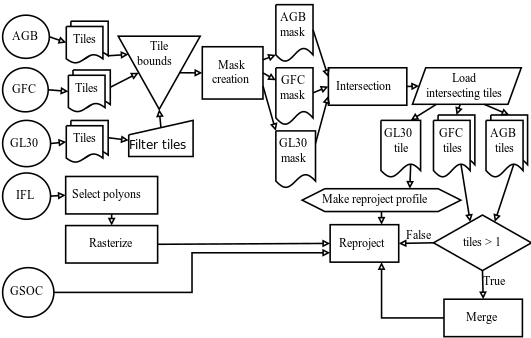
\includegraphics[scale=.97]{img/align}
			\caption[Raster and vector harmonization process]{\textbf{Raster and vector harmonization process:} For the multi-tiled datasets represented by the multi-document symbols a mask is created by extracting the tile bounds. Next, the intersection between these masks is determined to identify superimposing data and the corresponding tiles are loaded from the disk. GlobeLand30 (GL30) tiles are used as a template by creating the re-project profile and subsequently applying it to the intersecting tiles. From the Intact Forest Landscapes (IFL) layer only polygons within the re-project area are selected and subsequently converted to a raster layer. The Global Soil Organic Carbon Map as a single tile raster file with a spatial resolution of 1 km$^2$ is re-projected and re-sampled by the nearest-neighbor approach.}
			\label{fig:preprocessing_flowchart}
		\end{figure}

		The first exercise of the preprocessing algorithm is to detect all tiles covering the extent of our template tiles. First, we create for each multi-tiled dataset a polygon mask as \ac{SHP}. This mask contains the spatial extent of each tile within a dataset and as attribute the corresponding file identifier. If the dataset tiles are not in \ac{WGS84} the extracted bounds are subsequently reprojected to this \ac{CRS}. During the masking process, we recognized that the raster mosaic bounds of both \ac{GL30} datasets (2000 and 2010) generate re-projection errors. Further analysis revealed that all tiles located in \ac{UTM} zone 1 and 60 overflowed the maximum and minimum longitude coordinates of these zones. To solve this we excluded all tiles within \ac{UTM} zone 1 and 60 from further processing. Now, as the figure \ref{fig:preprocessing_flowchart} suggests we determine the intersection between these mask layers and group the intersecting tiles by our template tile. Next, we create for the template tile a re-projection profile (warp profile) and apply it subsequently to all intersecting tiles based on the following rules: if from one dataset more than one tile intersects merge them followed by re-projection; if only one tile intersects just re-project it. As introduced, the \ac{GSOCmap} consists only of one single tile with a spatial resolution of approximately 1 Km$^2$, so it must only be re-project and re-sampled by the nearest-neighbor approach. We select from the \ac{IFL} layer all polygons within our template warp profile and convert them to a raster layer where intact forest patches are coded by a one in an 8-bit unsigned integer. The last step of the alignment process is the rounding of the \ac{AISM} bounds to full integer degrees and a subsequent clipping of each tile to this rounded bounds. Finally, we create a polygon mask of our \ac{AISM} and store for each polygon as attributes the corresponding dataset tiles. This mask is used as a file index for the next algorithms. The figure \ref{fig:aligned_tiles} shows this mask and the extent of the harmonized dataset tiles. Each box in this figure highlights a raster tile stack of our \ac{AISM}. The advantage of this tiled approach is that we don't have to store 8 large raster files which cover the entire tropical zone and occupy a large amount of disk space and exceed the available memory if loaded for further processing. Further, this approach enables us to parallelize most of our further computations because each tile from our \ac{AISM} is a closed unit.
		\begin{figure}[!ht]
			\centering
			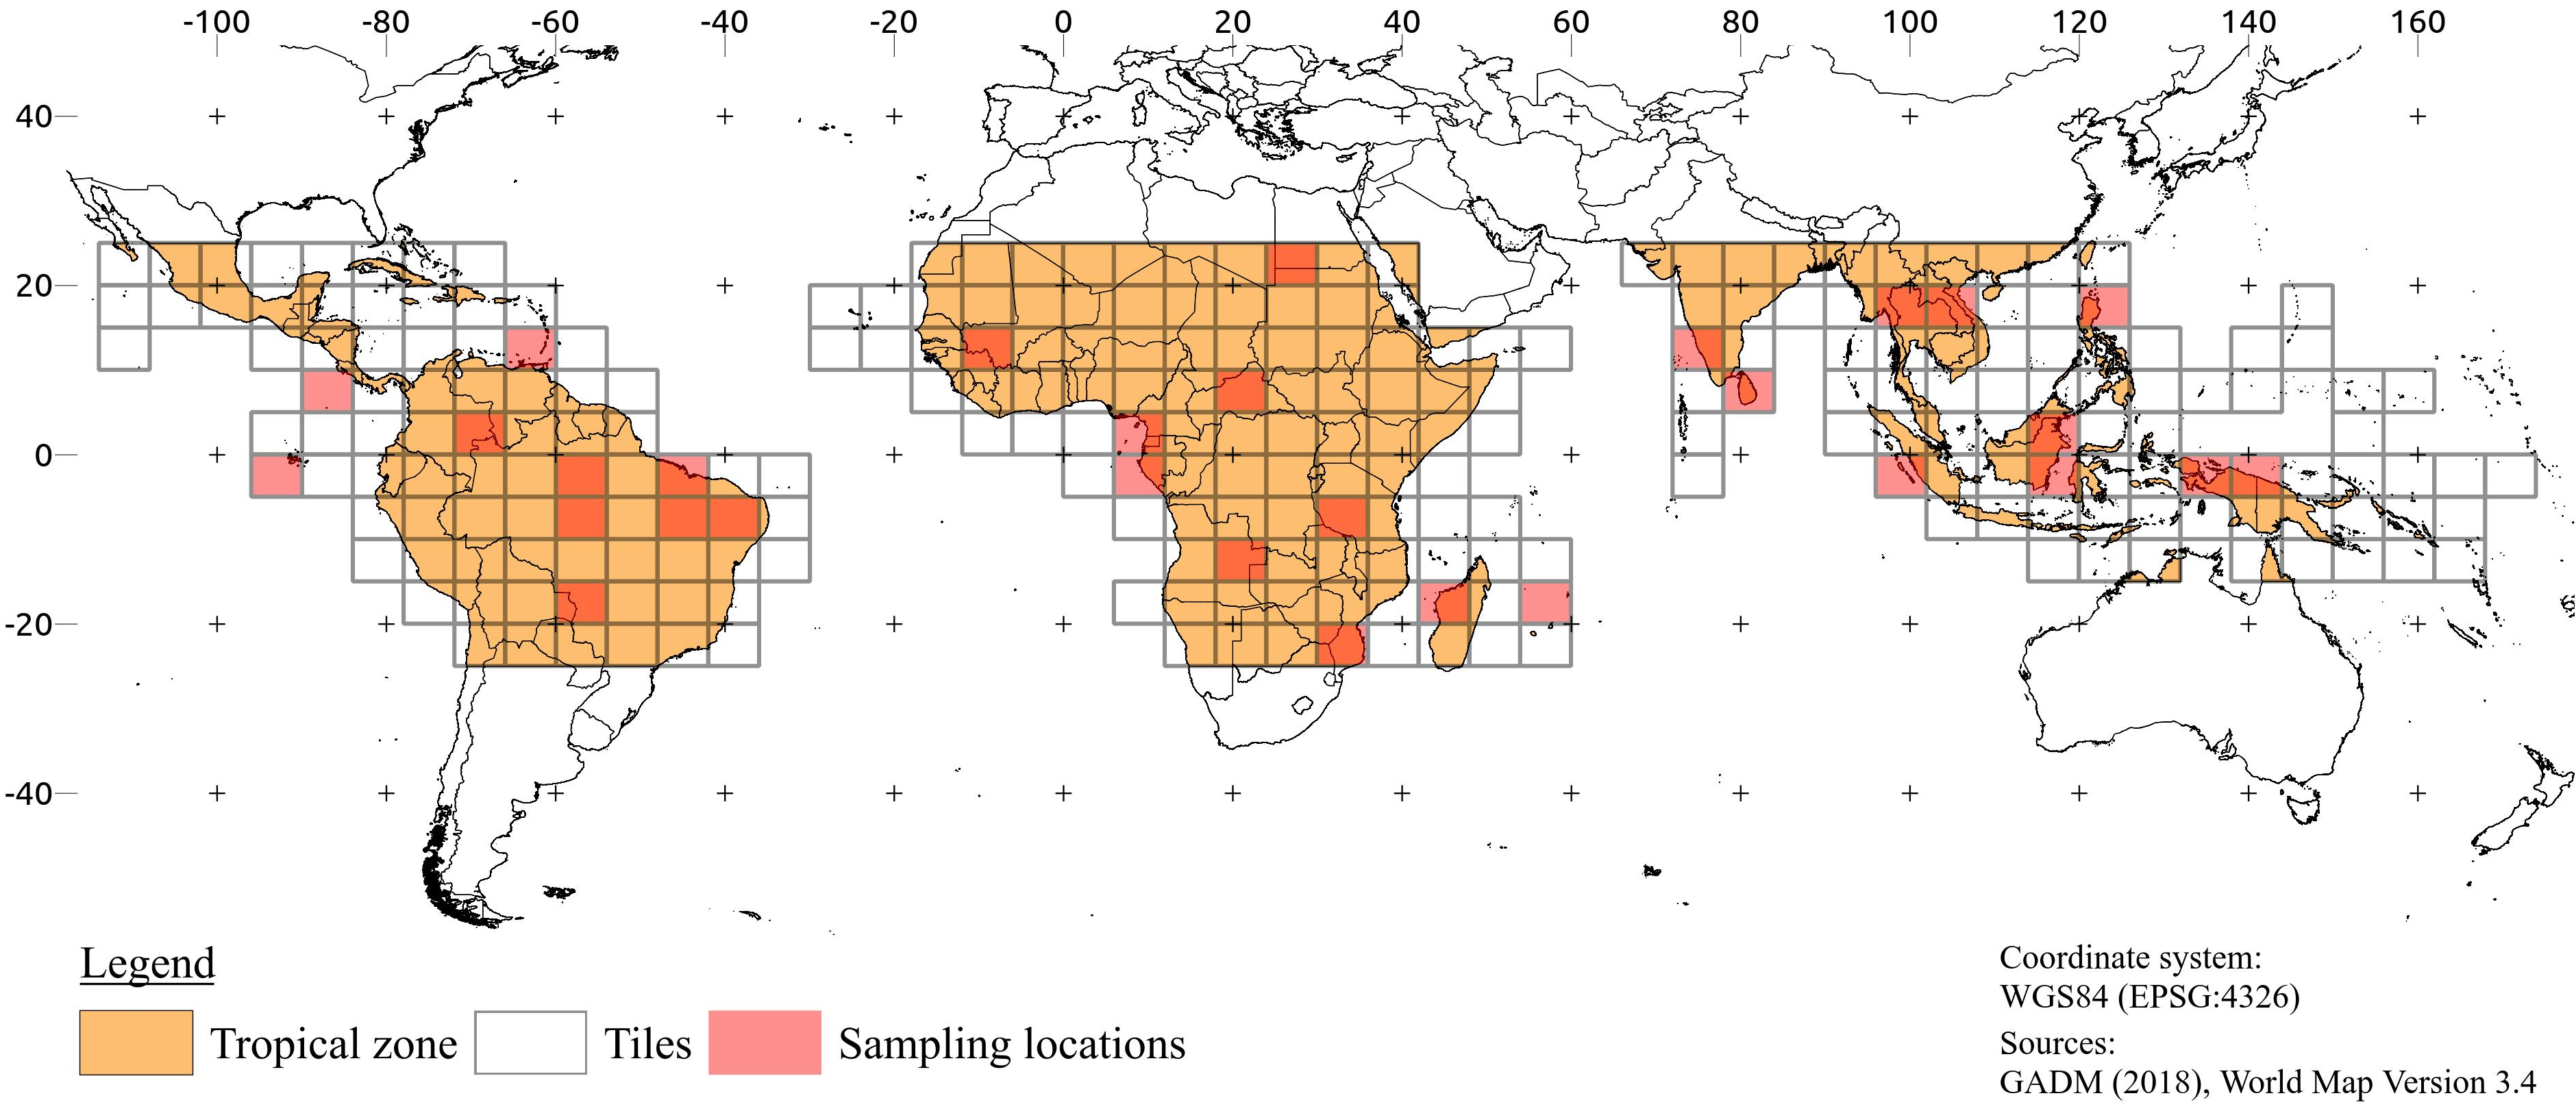
\includegraphics[scale=.96]{img/method_overview_frameless}
			\caption[Harmonized raster images and sampling locations]{\textbf{Harmonized raster images and sampling locations:} The map shows the location of the aligned multi-image stack tiles as black-framed, square-sized polygons. The sampling locations for accuracy assessment are represented in red, Countries within tropical range appear in orange. Vertical blue lines separate the tiles into the three continental regions Latin America, Africa, and Asia/Australia.}
			\label{fig:aligned_tiles}
		\end{figure}

	\subsection{Proximate deforestation drivers} 
		\subsubsection{Forest definition}
		\label{subsubsec:forest_definition}
			To determine the proximate drivers of deforestation we combined the information of the two datasets \ac{GFC} and \ac{GL30}. However, both differ in their definition of tree cover by canopy cover threshold as introduced in section \ref{sec:data}. \ac{GFC} detects tree cover over the entire canopy density interval of $(0,100]$, while the \ac{GL30} threshold is set to > 10 \%. To successfully extract stable land cover transformation by superimposing both layers we must first harmonize the tree cover definition of both strata. We hypothesize that if both layers agree on tree cover they should also agree if a transition to a non-forest state occurs. To harmonize both definitions we have the opportunity to vary the canopy density of \ac{GFC} to determine at which density class the similarity between them is at its maximum. Then, we use the examined maximum similarity canopy density to filter the tree cover loss and gain layer.

			To determine the similarity between \ac{GL30} 2000 and \ac{GFC} reference tree cover we used the \ac{JI}. The \ac{JI} or coefficient of community is a simple measure of similarity between two pairs of a binary population or a measure of the degree of spatial overlap between two images \citep{Sampat2009}. This index was first applied by \citeauthor{Jaccard1912} to compare distributions of rare alpine flora in 1912 \citep{Jaccard1912}, and since it is a widely used metric across multiple fields. If we compare two binary images, let $a$ be the magnitude where both images (Img$_1$, Img$_2$) have an agreement represented as a pixel value of one. Let $b$ the magnitude where Img$_1$ is zero and Img$_2$ is one, while $c$ represents the inverse expression. Finally, assume that $d$ is the magnitude of elements where both images are zero. The matrix in table \ref{tab:jaccard_matrix} shows that the computation of this coefficients $a$, $b$, $c$, and $d$ can be expressed as a set of boolean operations. Equation \ref{eq:jaccard_index} shows how the \ac{JI} is computed by substitute integer values for the variables. This computation can be reduced to two boolean operations for a major performance increase. The \ac{JI} is always within the closed interval $[0,1]$, where an index of one or zero means a complete similarity between both populations or a complete disagreement, respectively. The relationship between $a$ and \ac{JI} is near linear \citep{Shi1993}. The first step to compute the \ac{JI} for our raster images is to extract the tree cover from the \ac{GL30} 2000 land cover by setting all pixels with values $\neq$ 20 to zero and values $=$ 20 to one. Next, we extract from the \ac{GFC} reference tree-cover pixel values within the half-opened interval of the following canopy density classes and set them to one: $(0,100]$, $(10,100]$, $(20,100]$, and $(30,100]$. Therefore, we test four different tree cover definitions for \ac{GFC}. The first excludes canopy densities $\leq$ 0\%, the second $\leq$ 10\%, the third $\leq$ 20\%, and the fourth  canopy densities $\leq$ 30\%. We will refer to this \ac{JI} of different canopy density classes as JI$_0$, JI$_1$, JI$_2$, and JI$_3$. For all 269 tiles of our \ac{AISM}, we calculate the \ac{JI} existing between \ac{GL30} and \ac{GFC} for the four above-mentioned forest definitions by using equation \ref{eq:jaccard_index}. The algorithm is implemented in Python by using numpy's ability to perform boolean operations between large matrices. As parameters, the function expects two matrices with the same dimensionality in $R^{n*m}$ and a boolean indicating if the function should return the coefficient matrix as well. The previously described preprocessing steps are implemented as an extra function. This function requires as parameter two raster layers, a list of integer values to consider as \ac{GL30} forest cover (default is 20), and the lower bounds of the canopy density intervals to consider for computation.
			\begin{table}[ht]
				\centering
				\caption[Jaccard Index coefficient matrix]{\textbf{Jaccard Index coefficient matrix:} $a$ is the magnitude of agreement, $d$ is the magnitude of disagreement, $b$ and $c$ are the magnitudes of partial disagreements among both images. The computation of these coefficients can be expressed as boolean operations on matrices.}
				\label{tab:jaccard_matrix}
				\begin{tabular}{lccc}
					\hline
					& & \multicolumn{2}{c}{Img$_1$} \\
					& State & 1 & 0 \\\hline
					\multirow{2}{*}{\STAB{\rotatebox[origin=c]{90}{Img$_2$}}} & 1 & $a=|\mathbf{X_1} \land \mathbf{X_2}|$ & $b=|(\mathbf{X_1} \land \mathbf{X_2}) \oplus \mathbf{X_2}| $ \\ 
					& 0 & $c=|(\mathbf{X_1} \land \mathbf{X_2}) \oplus \mathbf{X_1}|$ & $d=|\neg ( \mathbf{X_1} \lor \mathbf{X_2})|$ \\\hline 
				\end{tabular}
			\end{table}
			\begin{equation}
			\label{eq:jaccard_index}
				JI = \frac{a}{a+b+c} = \frac{|\mathbf{X_1} \land \mathbf{X_2}|}{|\mathbf{X_1} \lor \mathbf{X_2}|}
			\end{equation}

			To optimize the overall tree cover similarity between both datasets we must test which canopy density class yields the highest agreement over our study extent. To test the significance of the difference between two correlated samples, we decided to apply the non-parametric Wilcoxon signed-rank test \citep{Wilcoxon1945}. This test requires paired data from the same population, at least an ordinal scale of measurement, each sample pair is independent, and the dependent variable can be expressed as a continuous probability \citep{Lowry2019}. Further, an advantage of this test is that we don't have to assume a normal distribution for our sample population. Our sample population fulfills these requirements.  The test procedure is implemented in R because this language is mainly intended for this kind of statistical analysis. We exported the computed \ac{JI} from our Python environment and applied a cross-testing in R. In our case, cross testing is defined as the test of all possible \ac{JI} combinations. Further, we applied a two- and one-sided Wilcoxon test because we want to examine if there is a significant difference and which direction has the similarity distribution. To address the higher probability of family-wise error in multiple comparisons we used a Holm correction. Before we applied the examination of the distribution we separated our population into three independent regions, namely Latin America, Asia/Australia, and Africa highlighted by the vertical blue lines in figure \ref{fig:dataset_tiles}. Latin America, Asia/Australia, and Africa comprised 82, 86, and 101 image tiles, respectively. Additionally, we excluded from the analysis all samples where JI$_0$ is zero because this tiles from our \ac{AISM} did not contain any pixels covered by trees. In Latin America, Asia/Australia, and Africa we excluded 6, 13, and 15 tiles. We tested continental differences in tree cover agreement to inspect regional dependencies and global differences. The results from the global testing are used to determine our definition of tree cover. Further, we compared differences of tree cover agreement between the continental regions by applying a Wilcoxon rank-sum test also known as Mann-Whitney U test. We applied a Benjamini and Hochberg correction to the test results.
 
		\subsubsection{Mapping of proximate deforestation drivers}
		\label{subsubsec:methods_proximate_deforestation_driver}
		%TODO cite natural earth
			Based on our forest definition developed in the previous section we want to classify all the tropical deforestation occurring within a canopy density of $(10,100]$ percent between 2001 till 2010. 

			Figure \ref{fig:driver_flowchart} shows an overview of the classification process, which we used to derive the \acp{PDD} of tropical tree cover loss. For classifying the \acp{PDD} we selected the following raster images from our \ac{AISM}: \ac{GFC} tree cover, \ac{GFC} annual losses, \ac{GFC} gain, and the \ac{GL30} \ac{LC} classification of 2010. Next, we apply to each raster image stack the following operations. From the reference tree-cover images, we select all pixels where the canopy density is within the half-open interval of $(10,100]$ percent and set them to one (true). The same exercise is applied on the annual losses stratum by setting all forest loss pixels within the time period 2001 till 2010 to one (true). After, both layers are combined with a logical AND operation to select our target deforestation pixels. Finally, we classify the pixels with a deforestation event by applying the Hadamard product (element-wise matrix multiplication) on the target deforestation layer and the \ac{GL30} \ac{LC} stratum. This operation basically creates a new image matrix by superimposing both layers. As output we obtain the exact \ac{LC} category of each deforestation pixel, which allow to understand what \ac{LC} transitions is driving tree cover loss in different regions. For classifying forest regrowth we filtered the \ac{GFC} gain layer to consider only tree cover gain within our target temporal resolution and target canopy density. After, the filtered stratum is aggregated with our classified deforestations by using the Hadamard product of both layers. The classification algorithm is implemented as a Python function which requires as parameters the previously named raster layers. Additionally the target canopy density and time period is freely selectable for experimental variations. The described filtering and aggregation steps are implements as binary matrix operations for fast processing of large data sizes by means of numpy.
			\begin{figure}[ht]
				\centering
				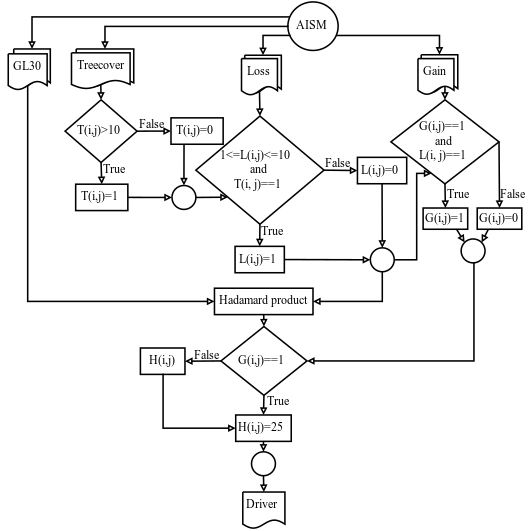
\includegraphics[scale=.88]{img/driver_flowchart}
				\caption[Classification of proximate deforestation drivers]{\textbf{Classification of proximate deforestation drivers:} For the classification of the proximate deforestation drivers the following layers are required: GlobeLand30 from 2010, Global Forest Change tree cover, annual losses, and gain. From the tree cover stratum we select all pixels within the canopy density interval $(10,100)]$. The tree cover mask is used to select the appropriate annual losses within the time interval $[2001,2010]$. To predict a land cover change after a deforestation event we use the Hadamard product (element-wise matrix multiplication). As output we obtain the exact land cover category of each deforestation pixel, which allow to understand what \ac{LC} transitions is driving tree cover loss in different regions.}
				\label{fig:driver_flowchart}
			\end{figure}

			Our \acp{PDD} classification scheme corresponds largely to the \ac{LC} schema of \ac{GL30} in table \ref{tab:gl30_classes}. We introduced regrowth (pixel code is 25) as a new \ac{LC} class from the \ac{GFC} gain datasets. The \ac{LC} type regrowth accounts for tree crops like oil palm plantations or forestry activities. Further, this class could be the natural regeneration of tree cover after using the area for other purposes like shifting agriculture. Tree cover loss classified as grassland account for the forest loss by the expansion of pastures for cattle ranching \citep{Graesser2015}. Tree cover loss classified as wetland and water is forest loss by inundation by lakes and rivers \citep{Sy2015}. Forest loss classified as forest by the \ac{GL30} layer could relate to false positives (predicts forest loss but there is no loss, type I error) of the \ac{GFC} loss layer. On the fact that the \ac{GFC} gain layer has a low overall accuracy and tends to underestimate tree cover gain the probability is higher that this pixels relate to false negatives (predicts no gain but there is gain, typ II error) of \ac{GFC} gain layer. We will relate to these pixels as miss-classifications that account for a mean miss-classification rate of 52\% (with large regional dependencies) if tree cover loss in the entire canopy density interval is considered for classification \citep{Seydewitz2017}. The next paragraph presents a approach to resolve this issue. 

			After classifying the proximate deforestation drivers we developed an approach to smooth the misclassified pixels based on \ac{LC} change probabilities. This means the algorithm tries to find for clusters of misclassified pixels and to reclassify them by finding the most frequent \acp{PDD} in the surroundings within a certain threshold. The first step of our reclassification is to cluster the misclassified pixels with the Hoshen-Kopelman algorithm \citep{Hoshen1998}. The clustering algorithm is implemented as a part of the GDAL (Geospatial Data Abstraction Library) library and can be called through the rasterio interface. For this project, we used the following parameters: connectivity 4 and a boolean mask where only pixels that relate to forest are set to true. Now the algorithm clusters only pixels which are set to true to one polygon. After, we created a squared-sized buffer with a side length of 500 m around the polygon centroid (the geometric midpoint of the polygon). Because \ac{WGS84} is not an equal area \ac{CRS} we must compute for each tile the buffer size separately. To compute the buffer size we used the Haversine formula in equation \ref{eq:haversine_function}. Let $d$ be the great-circle distance between two latitude, longitude pairs ($\varphi_n, \lambda_n$) and $r$ is the earth radius of approximately 6 378 137 meter. Because this computation is expensive we assumed that the pixel resolution is equal for an entire raster tile. After extracting the buffer we counted the most frequent class under exclusion of forest and no data pixels within the buffer. Finally, if a most frequent class is defined and we reassign this value to the cluster. The reclassification algorithm is implemented as a Python function which requires as parameters a \ac{PDD} raster image, a list of elements which should be interpreted as occupied cells for the clustering, pixel values which should be excluded from counting, the side length of the buffer, and the on-ground resolution. 
			\begin{equation}
			\label{eq:haversine_function}
				d = 2r\arcsin\left(
				\sqrt{
						\sin^2\left(\frac{\varphi_2-\varphi_1}{2}\right)+\cos\left(\varphi_1\right)\cos\left(\varphi_2\right)\sin^2\left(\frac{\lambda_2-\lambda_1}{2}\right)
				}
				\right)
			\end{equation}
			After preparing the predictions we aggregated our results on \acp{PDD} for country, continental and global scale by using the administrative bounds of the Natural Earth layer. To present our results as maps for the three continental regions we developed our own visualization approach that is explained in section \ref{subsec:methods_binning}.

		\subsubsection{Accuracy assessment}
			For examining the accuracy of our \ac{PDD} predictions we used a confusion matrix (also known as two-way frequency tables, error matrix or contingency tables). These matrices are commonly used for accuracy assessments of land cover classifications and enable the computation of marginal and conditional distributions \citep{Congalton1991,Foody2002}. Table \ref{tab:methods_confusion_matrix} shows a general model of a confusion matrix. The foundation for an accuracy assessment by means of a confusion matrix is a collection of ground-truth samples which can be compared with the class predictions of these samples produced by a classification algorithm. For the preparation of our accuracy assessment, we have to extract a collection of pixel samples with a deforestation occurrence from our proximate driver maps, which is also in this case the predictions. Next, we compose a set of ground-truth data for these predictions henceforth, references.
			\begin{table}[ht]
				\centering
				\caption[A general model of a confusion matrix]{\textbf{A general model of a confusion matrix:} $X_1$, ... , $X_n$ denote classification labels of two independent predictors. $x_{n,n}$ are the actual samples within each classification category. The diagonal values $x_{1,1}$, ..., $x_{n,n}$, highlight the agreement between both predictors. The remaining cell values account for the disagreement between the two predictors. $\sum$ column and row show the marginal distribution and N is the total number of samples.}
				\label{tab:methods_confusion_matrix}
				\begin{tabular}{lccccc}
					\hline
					& & \multicolumn{3}{c}{Reference} & \\
					& Cls & $X_1$ & $\cdots$ & $X_n$ & $\sum$ \\\hline
					\multirow{4}{*}{\STAB{\rotatebox[origin=c]{90}{Predict}}}
					& $X_1$ & $x_{1,1}$ & $\cdots$ & $x_{1,n}$ & $x_{1.}=
					\displaystyle\sum_{i=1}^{n} x_{1,i}$ \\ 
					& $\vdots$ & $\vdots$ & $\ddots$ & $\vdots$ & $\vdots$ \\ 
					& $X_n$ & $x_{n,1}$ & $\cdots$ & $x_{n,n}$ & $x_{n.}=\displaystyle\sum_{i=1}^{n}x_{n,i}$ \\\hline 
					& $\sum$ & $x_{.1}=\displaystyle\sum_{i=1}^{n}x_{i,1}$ & $\cdots$ & $x_{.n}=\displaystyle\sum_{i=1}^{n}x_{i,n}$ & $\sum\sum=N$ \\\hline
				\end{tabular}
			\end{table}

			To create our collection of ground-truth data we applied a stratified sampling. From all three continents we selected randomly 10 image tiles (figure \ref{fig:aligned_tiles}) and from each tile, we randomly sampled 200 pixels, which resulting to 6000 samples over the entire study region. The sampling is performed with our own raster sampling algorithm built in Python by means of the open source libraries numpy and rasterio. As mentioned in the previous section we superimpose two datasets and only a certain amount of pixels per tile are classified as a proximate driver. Therefore, the sampling algorithm should only draw samples from occupied/classified pixels without replacement. The algorithm expects as parameters a raster image, the total number of samples to draw, a list of pixel values which should be interpreted as occupied cells, the affine transformation matrix of the raster image, and a seed for the random number generator. If occupied cells are set the algorithm will create a binary mask where each occupied cell is set to one relative to the input raster image. Otherwise, it sets all pixel values greater or less than zero to one. After, the row and column coordinates of each one are extracted from the mask and converted to a flat list of coordinate tuples. Next, it draws the predefined number of samples from the list by a random order and uses the image coordinates to get the pixel value from the raster image. If an affine transformation matrix is provided the image coordinates are converted to real-world coordinates. The seed argument ensures that on every algorithm rerun the samples are drawn. For our sampling we set the parameters to the following values: samples 200, occupied pixels \ac{GL30} class values and 25 for regrowth, the affine matrix of the corresponding raster image, and the seed is 42. The per tile samples are stored as a CSV-file (Comma Separated Values).

			For the collection of ground-truth data, we used a visual interpretation of satellite and aerial imagery provided by Google Maps. We developed a small JavaScript web application to access the imagery via the Google Maps \ac{API}. The application expects as input a CSV file with the sampling coordinates. After upload of a sample file the user can cycle through the entries and the map jumps automatically to the coordinates of the sample. Now, a reference label can be assigned to the coordinates by visual interpretation of the imagery. We subsequently assigned to all 6000 samples a ground-truth label and downloaded the results as CSV.

			Finally, we developed a Python class to compute the confusion matrix. The constructor of the class requires a list of reference and prediction labels. With the provided arguments it creates the confusion matrix. Further, it computes the following marginal and conditional distributions: overall accuracy ($OvAc$), by dividing the sum of classification agreements by the sample total $N$ (equation \ref{eq:overall_accuracy}); the producer accuracy ($PAc_{.n}$), by dividing the category agreement by the column category total (equation \ref{eq:producer_accuracy}); the error of commission ($Com_{.n}$), by dividing the category disagreement by the column category total (equation \ref{eq:comission_error}); the user accuracy ($UAc_{n.}$), by dividing the category agreement by the row category total (equation \ref{eq:user_accuracy}); the error of omission ($Om_{.n}$), by dividing the category disagreement by the row category total (equation \ref{eq:omission_error}); and the Cohens Kappa by substituting equation \ref{eq:cohen_coefficient} and \ref{eq:overall_accuracy} into equation \ref{eq:kappa_coefficient}.
			\begin{equation}
			\label{eq:producer_accuracy}
				PAc_{.n} = \frac{x_{i,i}}{x_{.n}}
			\end{equation}
			\begin{equation}
			\label{eq:overall_accuracy}
				p_0=OvAc = \frac{\displaystyle\sum_{i=1}^{n}x_{i,i}}{N}
			\end{equation}
			\begin{equation}
			\label{eq:comission_error}
				Com_{.n} = \frac{FN_i}{x_{.n}}
			\end{equation}
			\begin{equation}
			\label{eq:user_accuracy}
				UAc_{n.} = \frac{x_{i,i}}{x_{n.}}
			\end{equation}
			\begin{equation}
			\label{eq:omission_error}
				Om_{n.} = \frac{FP_i}{x_{n.}}
			\end{equation}
			\begin{equation}
			\label{eq:cohen_coefficient}
				p_c = \frac{1}{N^2}\displaystyle\sum_{i=1}^{n} x_{.i} \cdot x_{i.}
			\end{equation}
			\begin{equation}
			\label{eq:kappa_coefficient}
				Kappa = \frac{p_0-p_c}{1-p_c}
			\end{equation}

	\subsection{Carbon losses}
		During the previous sections we developed an approach to map the change of tree cover driven by proximate causes like conversion to cropland. Now we can use these \ac{LC} change classes to approximate the carbon losses arising from these forest cover transitions. For this study, we focus on the carbon losses by biomass removal and by changes of soil carbon stocks. The first part of this section focuses on the estimation of carbon losses by biomass removal, while the second one focuses on the estimation of carbon losses arising from \ac{SOC} changes. 

		To obtain the gross carbon losses resulting from specific \ac{LC} changes we selected the following raster tiles from our \ac{AISM}: the \ac{AGB} stratum and our mapping of the proximate deforestation driver. By means of Python, we implemented a function which accepts as parameters two raster images, the area a pixel covers in $m^2$, and a list of proximate driver classes to consider as deforestation causes. We considered the following \ac{PDD} classes as deforestation: cropland, regrowth, grassland, shrubland, artificial, and bareland. The function computes the biomass losses by using equation \ref{eq:agb_formula}. Let $Y_{ij}$ be the \ac{AGB} in Mg biomass ha$^{-1}$ and $X_{ij}$ the \ac{PDD} at an pixel index $i,j$ obtained from a raster image matrix in $R^{N*M}$. Let $A$ be the area in ha a pixel covers for a certain image tile. This area is calculated by using the Haversine function from equation \ref{eq:haversine_function}. Let $AGB_{tile}$ be the cumulative aboveground biomass losses emitted by the removal of tree cover per raster tile. Then this value can be obtained by taking the sum of the product of $Y_{ij}$ and $f(X_{ij})$. The piecewise function $f$ only evaluates to one if the \ac{PDD} is within our set of classes we want to consider as deforestation causes. To asses the total biomass density per tile ($TB_{tile}$) we used equation \ref{eq:bgb_formula} from \citet{Saatchi2011}. To obtain the gross carbon loss (Mg C ha$^{-1}$) by biomass removal through the deforestation by \acp{PDD} we aggregated the sum of $TB_{tile}$ and multiplied it by 0.5 for the regions Latin America, Asia/Australia, and Africa \citep{Achard2014}.
		\begin{equation}
		\label{eq:agb_formula}
			AGB_{tile} = A\displaystyle\sum_{i=0}^{N}\displaystyle\sum_{j=0}^{M} f(X_{ij})Y_{ij}
		\end{equation}
		\begin{equation}
		\label{eq:bgb_formula}
			TB_{tile} = AGB_{tile} + 0.489*AGB_{tile}^{0.89}
		\end{equation}
		To obtain the gross carbon losses by the change of soil organic carbon content we selected the following raster tiles from our \ac{AISM}: the \ac{IFL} stratum, the \ac{GSOCmap}, and our \acp{PDD} layer. We decided to estimate the \ac{SOC} losses for two different scenarios. In scenario one (SC$_1$) we assume that all tree covered areas concerned by a land cover change are primary forests. For scenario two (SC$_2$) we used the \ac{IFL} stratum to determine the forest type. If \ac{LC} changes occur within an \ac{IFL} patch we consider it concerns primary forest, otherwise it is considered as secondary forest. The \ac{SOC} losses of both scenarios can be computed by equation \ref{eq:soc_formula}. Let $X_{ij}$ be the \ac{PDD} from our deforestation driver layer, $Y_{ij}$ the forest type determined by the \ac{IFL} stratum, and $Z_{ij}$ the \ac{SOC} in Mg C ha$^{-1}$ determined by \ac{GSOCmap} at a pixel with the coordinates $i,j$ obtained from a raster image matrix in $R^{N*M}$. Let $A$ be the area in ha that a pixel covers for a certain image tile. This area is calculated by using the Haversine function from equation \ref{eq:haversine_function}. Let $SOC_{tile}$ be the cumulative soil organic carbon losses emitted by the change of forest to another land cover type. Then this value can be obtained by taking the sum of the product of $Z_{ij}$ and $h(X_{ij}, Y_{ij})$. The piecewise function $h$ returns the mean soil organic carbon change and the standard error in respect to the forest type and proximate driver class. The mappings of driver classes and forest type for both scenarios are shown in table \ref{tab:scenario}. This algorithm is implemented by means of Python. The function needs as parameter the required layers, the area a pixel covers in $m^2$, an identifier for the forest type, and if the standard error should be included during the computation of the emission. If the \ac{IFL} stratum is provided the algorithm will rely on this layer to determine the forest type, otherwise it uses forest type identifier. To obtain the gross \ac{SOC} losses resulting from the \ac{LC} changes we aggregated the sum of $SOCE_{tile}$ for the regions Latin America, Asia/Australia, Africa, and globally. 
		\begin{equation}
		\label{eq:soc_formula}
			SOC_{tile} = A\displaystyle\sum_{i=0}^{N}\displaystyle\sum_{j=0}^{M} h(X_{ij}, Y_{ij})Z_{ij}
		\end{equation}
		\begin{table}[ht]
			\centering
			\caption[Soil organic carbon change in relation to proximate deforestation driver]{\textbf{Soil organic carbon change in relation to proximate deforestation driver:} Standard errors of the soil organic carbon change factors are denoted in table \ref{tab:soc_factors}.}
			\label{tab:scenario}
			\begin{tabular}{lrrrrr}
				\hline
				& \multicolumn{5}{c}{Proximate driver class} \\\cline{2-6}
				Forest type & Cultivated & Regrowth & Grassland & Shrubland & Bareland \\
				\hline
				Primary & .252 & .086 & .121 & .121 & .121 \\
				Secondary & .213 & - & .064 & .064 & .064 \\
				\hline
			\end{tabular}
		\end{table}

	\subsection{Ecosystem service values}
	\label{subsec:methods_esv}
		For a comprehensive insight of the \ac{ESV} dynamics, we quantified the loss of \ac{ESV} from tree cover depletion within the tropical zone. This loss of forest cover is frequently followed by a transition to other land cover types, which is expressed through our \acp{PDD}. These transitions can be interpreted as a gain or loss of \acp{ESV} and are computed subsequently. Finally, to give an insight into the overall trend of both \ac{ESV} dynamics we determined the balance among the monetary loss and gain. We estimate the \acp{ESV} dynamics by considering three different approaches found in the literature \citep{Costanza2014,Groot2012,Siikamaki2015}. The first part of this section describes our approach to determine the \ac{ESV} loss, followed by the method to obtain the gain in monetary units, and finally we explain how to derive the balance between both values. To compute these \ac{ESV} dynamics we used the benefit transfer approach.

		By applying equation \ref{eq:esv_loss} we compute the gross \ac{ESV} loss from the loss of tropical tree cover for the entire set of our \ac{AISM}. Let $X_{ij}$ be the \acp{PDD} from our prediction at a pixel with the index $i,j$ (image coordinates) obtained from a raster image matrix in $R^{N*M}$. Let $ESV_{Forest}$ be the \ac{ESV} of tropical forest from one of our selected source datasets from table \ref{tab:esv_mapping}. Let $A$ be the area in ha a pixel covers for a certain image tile. The pixel area is calculated by using the Haversine function from equation \ref{eq:haversine_function}. Let $ESV_{loss,tile}$ be the cumulative loss in \ac{ESV} for a certain tile from our \ac{AISM}. Then this value can be determined by adding the product of $f(X_{ij})$ and $ESV_{Forest,Dataset}$. The function $f$ returns only a one if the \ac{PDD} is considered as deforestation by the mapping in table \ref{tab:esv_mapping}. The computation of \ac{ESV} loss is implemented as a Python function. The function accepts as parameters a raster image of \ac{PDD} predictions or a pandas data frame object. Further, the function requires as parameter the area a pixel covers in ha and the monetary value of tropical forest. Additionally, the function requires a list of \ac{PDD} classes considered as the loss of tropical forest cover. We considered the following \ac{PDD} classes as anthropogenic tree cover loss: cultivated land, regrowth, grassland, shrubland, artificial surfaces, and bareland as table \ref{tab:esv_mapping} suggests. We excluded pixel classified as forest by our \ac{PDD} prediction because within this class we are uncertain if a deforestation event occurred. Further, we excluded transitions of tree cover to wetland or water because we assume this \ac{LC} changes are largely driven by natural causes.
		\begin{equation}
		\label{eq:esv_loss}
			ESV_{loss,tile} = A\displaystyle\sum_{i=0}^{N}\displaystyle\sum_{j=0}^{M} f(X_{ij})ESV_{Forest,Dataset}
		\end{equation}
		\begin{table}[ht]
			\centering
			\caption[Ecosystem service values corresponding to proximate deforestation drivers]{\textbf{Ecosystem service values corresponding to proximate deforestation drivers:} The monetary values are given in 2007 Int'I\$ y$^{-1}$ ha$^{-1}$, also known as Geary-Khamis Dollar. Mapping of biome types to proximate deforestation drivers have the following schema: cultivated to cropland biome, regrowth to tropical forest biome, grassland to grassland biome, and artificial surfaces to the urban biome. The abbreviations in dataset column refer to the following publications: \citet{Costanza2014} (Co), \citet{Groot2012} (Dg), and \citet{Siikamaki2015} (Wb)}
			\label{tab:esv_mapping}
			\begin{tabular}{lrrrrrr}
				\hline
				& \multicolumn{6}{c}{Proximate deforestation driver class} \\\cline{2-7}
				Dataset & Cultivated & Regrowth & Grassland & Shrubland &  Artificial & Bareland \\
				\hline
				Co & 5567 & 5382 & 4166 & - & 6661 & - \\
				Dg & - & 5264 & 2871 & - & - & - \\
				Wb & - & 1312 & - & - & - & - \\
				\hline
			\end{tabular}
		\end{table}
		To estimate the gain in \ac{ESV} from the transition of tropical forest to other land cover classes per \ac{AISM} tile we applied equation \ref{eq:esv_gain}. Let $X_{ij}$ be the \ac{PDD} from our prediction at a pixel with the index $i,j$ obtained from a raster image matrix in $R^{N*M}$. Let $A$ be the area in ha a pixel covers for a certain image tile. The pixel area is calculated by using the Haversine function from equation \ref{eq:haversine_function}. Let $ESV_{gain,tile}$ be the cumulative gain of \ac{ESV} per tile. Then this value can be determined by taking the sum of $h(X_{ij})$. The function $h$ returns for a selected \ac{PDD} class the corresponding monetary value. The algorithm is implemented in Python. The function accepts as parameters a raster image of \ac{PDD} predictions or a pandas data frame object. Further, the function requires as parameter a mapping of \acp{ESV} to \ac{PDD} classes from table \ref{tab:esv_mapping}. Additionally, the function can be called with a exclude list of \ac{PDD} classes.
		\begin{equation}
		\label{eq:esv_gain}
			ESV_{gain,tile} = A\displaystyle\sum_{i=0}^{N}\displaystyle\sum_{j=0}^{M} h(X_{ij})
		\end{equation}
		By applying equation \ref{eq:esv_balance} we compute the \ac{ESV} balance for each tile of our \ac{AISM}. Let $ESV_gain$ be the total \ac{ESV} gain per continental region and $ESV_{loss}$ the total \ac{ESV} loss per region. Then the \ac{ESV} balance $ESV_{balance}$ can be obtained by the difference of $ESV_gain$ and $ESV_{loss}$.
		\begin{equation}
		\label{eq:esv_balance}
			ESV_{balance} = ESV_{gain} - ESV_{loss}
		\end{equation}
		For our study we aggregated the \ac{ESV} loss, gain, and net balance dynamics on two spatial ranges with the following extent: per continental region (Latin America, Africa, and Asia/Australia) highlighted in figure \ref{fig:aligned_tiles} and on global scale.

	\subsection{Binning analysis and visualization}
	\label{subsec:methods_binning}
	%TODO cite natural earth
	%TODO image change y_2 to y_1
	%TODO image change equations to explain
		The previous sections, were focused on the exercise of creating large scale, spatially-explicit estimations of \ac{LC} changes and its impact on both \ac{GHG} emissions and \acp{ESV}. Now, an appropriate method must be developed to analyze and visualize these spatial explicit datasets. Due to the fine resolution of the raster images and the large area of our study extent we must handle a large $N$ (many samples). Therefore we high dimensional data and a complex relationship between the samples as a consequence of the large $N$ \citep{Carr1990}. Raster image maps can be interpreted as multivariate scatter plots. In our case this scatter plot has the three dimensions $x$ is the longitude, $y$ the latitude coordinate of a pixel, and $z$ is the nominal scaled pixel value in case of the \acp{PDD} layer. Drawing scatter plots with large multidimensional $N$ commonly leads to over-plotting and hidden point densities \citep{Carr1987}. Additionally, it is to assume that the distribution of \ac{PDD} is not equally distributed over the entire study extent. Hence, there should be regions with sparse data densities and with high densities but our goal is to visualize land cover changes on a continental level. As mentioned the ground resolution of one pixel covers an area of approximately 30x30 m and as an example, while the bounding box of Latin America covers an area of $5*10^7$ km$^2$. The large frame size as well the unequal distributed data leads to the issue that only large scale land cover changes are representable and small scale isolated changes remain hidden.

		Our goal should be to develop a process to solve the representation issues and to generate satisfying maps. In the case of raster data, one option could be a re-sampling to a coarser on-ground resolution. This approach may solve the over-plotting, the resolution issues, and normalize unequal distributed data. For nominal-scaled data the commonly used re-sampling methods are nearest neighbor or majority wins. However, both approaches are not appropriate because they would negate spatial patterns and eliminate important land cover class frequency distributions. Another well-accepted method is binning of spatially explicit data with a regular polygon that can tessellate the plane \citep{Carr1992}. Polygon tessellations provide numerous opportunities for presenting multivariate statistical and visual summaries. The scale of a polygon may be used to visualize pixel densities within the bounds and a color gradient may be used to prepare a choropleth map for nominal or ordinal scaled data. Additionally, the interior of a polygon may be used to prepare a pie chart. Hence, binning enables convenient visualization of multidimensional data. For preparing a regular tessellation only three types of convex polygons can be used to tessellate the plane: squares, equilateral triangles, and hexagons \citep{Carr1992}. Square tessellations are the most common method for binning and visualizing spatial data. Every raster image is already a square tessellation of the mapped object and most of the image processing algorithms are focused on squares. However, hexagon mosaic maps have two major advantages over square tessellations: visual appeal and representational accuracy. Binning of data by a square or hexagon mosaic creates visual lines. These lines compete with the data-generated patterns. Since humans have a strong visual response to horizontal and vertical lines, the line artifacts of square tessellations can be distracting and should be avoided. In light of this, we decided to use hexagon mosaic maps to represent the visual and statistical results of our study. For bivariate representations, we select the combination of scaling and color gradient. Multivariate data is visualized by hexagonal pie charts as choropleth cartogram. The following paragraphs describe our algorithmic approach to create these mosaic maps. We used Python and the open source library shapely to implement our algorithms.

		The first step to construct a hexagon tessellation is to define the vertices of the polygon. There are two common orientations of hexagons in $R^2$, flat topped and pointy topped. For our hexagon construction we decided to use pointy-topped polygons. For flexibility our algorithm accepts one out of four parameter to construct a hexagon polygon. The unit of the parameter is always in map units. Let $D$ be the long diagonal (diameter of the circumscribing circle), $d$ the short diagonal (diameter of the inscribed circle), $A$ the area the hexagon should cover, and $e$ the edge length of a hexagon. Let $R$ be the radius of the circumscribing circle. Then $R$ can be obtained by applying equation \ref{eq:hexagon_parameter} with one out of the parameter set $D$, $d$, $A$, or $e$. $R$ is used to compute the center vector $\vec{m}=<c_x, c_y>$ of the polygon by applying equation \ref{eq:hexagon_center_x} and \ref{eq:hexagon_center_y}. The polygon center is always located in the first quadrant of the Cartesian coordinate system. Now, by using $R$, $c_x$, and $c_y$ we can obtain $\mathbf{H}$, the anti-clockwise orientated vertex matrix of a hexagon. The construction of a hexagon by using the introduced method is shown in the left bottom corner of figure \ref{fig:hexagon}. The next paragraph describes how we derive a tessellation from the constructed hexagon.
		\begin{equation}
		\label{eq:hexagon_parameter}
			R = \frac{\sqrt{2A}}{\sqrt[4]{27}} = \frac{D}{2} = \frac{d}{\sqrt{3}} = e
		\end{equation}
		\begin{equation}
		\label{eq:hexagon_center_x}
			c_x = \frac{R\sqrt{3}}{2} 
		\end{equation}
		\begin{equation}
		\label{eq:hexagon_center_y}
			c_y = R
		\end{equation}
		\begin{equation}
		\label{eq:hexagon_matrix}
			\mathbf{H} =
			\begin{bmatrix}
				0 & c_x & 2c_x & 2c_x & c_x & 0 \\
				R\sin\left(\frac{7\pi}{6}\right) + c_y & 0 & R\sin\left(\frac{11\pi}{6}\right)+c_y & R\sin\left(\frac{\pi}{6}\right)+c_y & 2R & R\sin\left(\frac{5\pi}{6}\right)+c_y \\
				1 & 1 & 1 & 1 & 1 & 1
			\end{bmatrix}
		\end{equation}
		\begin{figure}[ht]
			\centering
			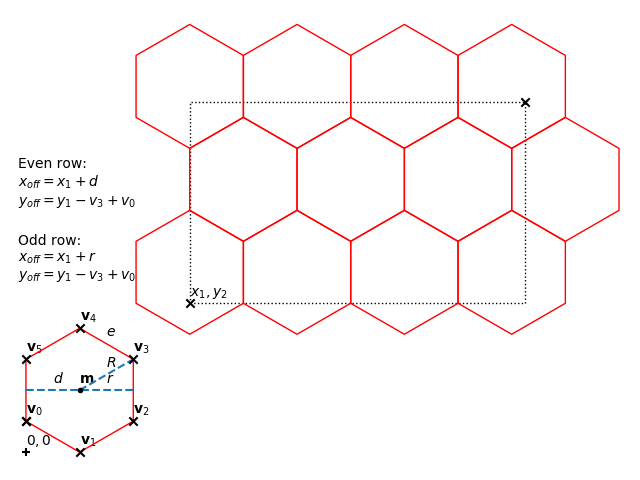
\includegraphics[scale=.66]{img/hexagons}
			\caption[Hexagon tessellation]{\textbf{Hexagon tessellation:} Located at the left bottom corner in red is a hexagon defined by its geometric properties: the 6 vertex vectors \{$\vec{v_0},...,\vec{v_5}$\} (black crosses), with center vector $\vec{m}$, edge length $e$, $R$ radius of the circumscribing circle, $r$ radius of the inscribed circle and $d$ the short diagonal (diameter of the inscribed circle). Top right black dotted box are the bounds of an area which is tessellated by a hexagon grid in red. Each grid cell is translated from the origin hexagon at its position by computing the $x_{off}$ and $y_{off}$ offset with the presented equations at the left-hand side of the grid. }
			\label{fig:hexagon}
		\end{figure}
		To create a polygon grid of a plane image we must align several hexagons to cover the image. For our tessellation algorithm we use the vertex matrix $\mathbf{H}$ computed by the previously described approach and subsequently translate it to its position within the grid. We expect to receive the bounds matrix $\mathbf{B}$ of the raster image, which should be tessellated by hexagons, equation \ref{eq:hexagon_bounds}. Let $x_1$, $y_1$ be the left bottom corner coordinates and $x_2$, $y_2$ the right top corner coordinates of an image. Let $x_{off}(0)$, $y_{off}(0)$ in equation \ref{eq:hexagon_x_off_start} and \ref{eq:hexagon_y_off_start} be the initial coordinates for creating a polygon grid over a plane. Then we can obtain $x_{off}(n+1)$, the $x$ coordinates for even rows by applying equation \ref{eq:hexagon_x_off_even} and $x_{off}(n+1)$, the $x$ coordinates for odd rows by equation \ref{eq:hexagon_x_off_odd}. $r$ is the radius of an inscribed circle in a hexagon and can be obtained by dividing $d$ by 2. Then $\mathbf{H}$ can be translated to the vertex matrix $\mathbf{T}$ by applying the dot product of an affine transformation matrix and $\mathbf{H}$, equation \ref{eq:hexagon_translate}.
		\begin{equation}
		\label{eq:hexagon_bounds}
			\mathbf{B} =
				\begin{bmatrix}
				x_1 & x_2 \\
				y_1 & y_2
			\end{bmatrix}
		\end{equation}
		\begin{equation}
		\label{eq:hexagon_x_off_start}
			x_{off}(0)=x_1
		\end{equation}
		\begin{equation}
		\label{eq:hexagon_y_off_start}
			y_{off}(0)=y_1
		\end{equation}
		\begin{equation}
		\label{eq:hexagon_x_off_even}
			x_{off}(n+1)=x_{off}(n)+d
		\end{equation}
		\begin{equation}
		\label{eq:hexagon_x_off_odd}
			x_{off}(n+1)=x_{off}(n)-r+d
		\end{equation}
		\begin{equation}
		\label{eq:hexagon_y_off}
			y_{off}(n+1)=y_{off}(n)-v_{0,2}+v_{3,2}
		\end{equation}
		\begin{equation}
		\label{eq:hexagon_translate}
		\mathbf{T} =
			\begin{bmatrix}
				1 & 0 & x_{off}(n) \\
				0 & 1 & y_{off}(n) \\
				0 & 0 & 1
			\end{bmatrix} \circ \mathbf{H}
		\end{equation}
		To construct a hexagonal pie chart we have to split the polygon into horizontal pieces in relation to a certain ratio. Thus, a horizontal split is required, whose $x$ and $y$ coordinates are located on the on the polygons convex hull. We compute the $y$ coordinates of the horizontal split line for the ratio $P$ by applying equation \ref{eq:hexagon_ratio}. Where $y_1$ and $y_2$ refer to the lower and upper $y$ coordinate of the hexagon bounding box. To compute the $x$ coordinates of the split line we applied a analytical solution. The shape of a hexagon can be expressed as a piecewise function of six linear functions, if the bounding box and the $R$ radius of the circumscribing circle is defined. By inverting this piecewise function and substituting $R$ (radius), $x_1$ (left x coordinate of the bounding box), $x_2$ (right x coordinate of the bounding box), $y_1$ (lower y coordinate of the bounding box), $y_2$ (upper y coordinate of the bounding box), and $y$ (y coordinate of the split line) we get both $x$ coordinates $g^{-1}(y)$ and $g^{-1}(y)$ of the split line $\mathbf{L}$ shown in equation \ref{eq:hexagon_left_intersection}, \ref{eq:hexagon_right_intersection}, and \ref{eq:hexagon_split_line}.
		\begin{equation}
		\label{eq:hexagon_ratio}
			y = \frac{P(y_2-y_1)}{100} + y_1
		\end{equation}
		\begin{equation}
		\label{eq:hexagon_left_intersection}
			f^{-1}(y) =
			\begin{cases} 
				-\frac{y - y_1}{\tan{(\frac{\pi}{6}})} + \frac{x_1 + x_2}{2} & \text{if } y_1 \le y < y_1 + R\sin{(\frac{5\pi}{6})} \\
				x_1 & \text{if } y_1 + R\sin{(\frac{5\pi}{6})} \le y < R(\sin{(\frac{5\pi}{6})} + 1) \\
				\frac{y - y_2}{\tan{(\frac{\pi}{6}})} + \frac{x_1 + x_2}{2} & \text{if } R(\sin{(\frac{5\pi}{6})} + 1) \le y \le y_2
			\end{cases}
		\end{equation}
		\begin{equation}
		\label{eq:hexagon_right_intersection}
			g^{-1}(y) = 
			\begin{cases} 
				\frac{y - y_1}{\tan{(\frac{\pi}{6}})} + \frac{x_1 + x_2}{2} & \text{if } y_1 \le y < y_1 + R\sin{(\frac{5\pi}{6})} \\
				x_2 & \text{if } y_1 + R\sin{(\frac{5\pi}{6})} \le y < R(\sin{(\frac{5\pi}{6})} + 1) \\
				-\frac{y - y_2}{\tan{(\frac{\pi}{6}})} + \frac{x_1 + x_2}{2} & \text{if } R(\sin{(\frac{5\pi}{6})} + 1) \le y \le y_2
			\end{cases}
		\end{equation}
		\begin{equation}
		\label{eq:hexagon_split_line}
			\mathbf{L} =
			\begin{bmatrix}
				f^{-1}(y) & g^{-1}(y) \\
				y & y
			\end{bmatrix}
		\end{equation}
		By using our hexagonal approach we prepared four different cartogram categories: hexagonal country boundaries, tree cover and canopy density cartogram, tree cover loss cartogram, and the \acp{PDD} cartogram. We processed each continental region as single map to obtain an appropriate image resolution. First, we generated a hexagon grid for each continent. Whereas, each grid cell cover an area of 0.5 x 0.5 decimal degrees, which translates to approximately 49 thousand km$^2$ at the equator. Next, we used the grid to construct the four different cartograms. For the tree cover maps we computed the total area covered by trees within a polygon and divide by the total area of the hexagon to determine the scaling. Additionally we aggregate the canopy density within a hexagon by applying the arithmetic mean. To arrange the tree cover loss maps we used our \ac{PDD} products. We computed the loss area within each hexagon for the following \ac{PDD} classes: cultivated land, regrowth, grassland, shrubland, artificial surfaces, and bareland. To determine the polygon scaling we divided the per hexagon loss area by the highest observed loss within a continental region. Forest cover, losses, and hexagon areas are computed by applying the Haversine equation \ref{eq:haversine_function}. To prepare the continental cartograms for the \acp{PDD} of tropical forest cover we counted the frequency of each \ac{PDD} class within a hexagon interior. After, we used our hexagon segmentation algorithm to split the polygon in relation to the relative frequency of a \ac{PDD} class. Whereas the order of appearance is decreasing. The \ac{PDD} with the largest frequency is the first quantity in the hexagons interior. The hexagonal country boundaries are an additional overlay to separate the hexagons to their corresponding countries visually. The country boundaries are an approximation of the real country boundaries in relation to the Natural Earth Map shown in the figures \ref{fig:americas_hexagonal_appendix}, \ref{fig:asia_hexagonal_appendix}, and \ref{fig:africa_hexagonal_appendix} in the appendix \ref{ch:appendix_a}.  